\chapter{Probability}
\label{chap:probability}

\begin{quotation}
      \textit{``Probability theory is nothing but common sense reduced to calculation.'' - Pierre-Simon Laplace}
\end{quotation}

Probability theory and statistics can be traced back to as early as the 17th century. In 1718,~\citeauthor{ref:demoivre:1718}~\cite{ref:demoivre:1718} published the \textit{Doctrine of of Chance}; a book that is widely seen as the first published book on probability theory. In 1763, Thomas Bayes~\cite{ref:bayes:1763} published an article titled \textit{An Essay towards solving a Problem in the Doctrine of Chances} where the first version of Bayes' Theorem was introduced. It is from this theorem that the \ac{BHH} was named after.

Probability theory and statistics play a vital role in the \ac{ML} space. A lot of constructs that arise in \ac{ML} originate from the fields of statistics and probability theory. There are many examples of how these two fields overlap. In 1991,~\citeauthor{ref:denker:1991},~\cite{ref:denker:1991} proposed a way to transform \ac{ANN} outputs to probability distributions. In 1993,
\citeauthor{ref:neal:1993}~\cite{ref:neal:1993} developed the first \ac{MCMC} sampling algorithm for Bayesian \acp{NN}. These are just a  few examples of how the fields of probability theory, statistics and \ac{ML} overlap.

So far the reader has been provided with the problem statement and goals of this dissertation in Chapter \ref{chap:introduction} and a detailed literature study and background information on \acp{ANN} was provided in Chapter \ref{chap:anns}. This chapter aims to provide the reader with the necessary background information on probability theory and statistics. These are big fields and focus is put on the elements that are required to formulate the proposed \ac{BHH}. The remainder of the chapter is structured as follows.

\begin{itemize}
      \item \textbf{Section \ref{sec:probability:overview}} gives a brief overview of what probability is and how it is used.

      \item \textbf{Section \ref{sec:probability:multiple_events}} presents the concept of conditional probability.

      \item \textbf{Section \ref{sec:probability:multiple_events}} presents the two laws of probability related to the intersection and union of multiple events.

      \item \textbf{Section \ref{sec:probability:cond_probability}} introduces conditional probability.

      \item \textbf{Section \ref{sec:probability:bayes_theorem}} introduces Bayes' Theorem, the fundamental theorem upon which the \ac{BHH} is built.

      \item \textbf{Section \ref{sec:probability:probability_distributions}} presents relevant probability distributions.

      \item \textbf{Section \ref{sec:probability:conjugate_priors}} presents the conjugate prior probability distributions for the probability distributions provided in Section \ref{sec:probability:probability_distributions}.

      \item \textbf{Section \ref{sec:probability:bayesian_statistics}} presents \textit{Bayesian} statistics. Brief discussions follow on the \textit{frequentist} view and \textit{Bayesian} view of probability. It is shown how Bayes' Theorem can be used to apply Bayesian statistics a alternative mechanism to do inference. Detailed discussions follow on \index{Bayesian optimisation}Bayesian optimisation methods such as \index{Bayesian analysis}\textit{Bayesian analysis}.

      \item Finally, a summary of the elements discussed in this chapter is provided in \textbf{Section \ref{sec:probability:summary}}.
\end{itemize}




\section{Overview}
\label{sec:probability:overview}


In everyday conversation, the term \textit{probability} is a measure of one's belief in the occurrence of a future event~\cite{ref:wackerly:2014}. Probability is a necessary tool used in many fields including physics, biology, chemistry and computer science. These fields contain many cases that generate observations that can not be predicted with absolute certainty~\cite{ref:wackerly:2014}. Probability can be be inferred and confirmed through past events. These events are referred to as \textit{random} or \textit{stochastic} events. The probability that a certain event $A$ might occur is denoted $P(A)$. Although these random events cannot be predicted with absolute certainty, the relative frequency with which they occur over many trials if often remarkably stable. Consider flipping an unbiased, fair coin. The coin has two possible outcomes. From this, one can conclude that each side has a $\frac{1}{2}$ or $50\%$ chance of occurring. In statistics, the decimal probability notation is used where $0 <= P(A) <= 1$. Suppose the fair coin is thrown 10 times, one is not guaranteed to observe $0.5$ heads and $0.5$ tails. There is is some probability, although small, that the coin might fall on heads $0/10$ times. The probability of such an event occurring is $0.0009765625$. The \ac{CLT} shows that the normalised sum of events tends toward a normal distribution with a mean value of $0.5$ if the number of events observed $N$, is large~\cite{ref:wackerly:2014}. The larger the value of $N$, the higher the confidence of mean probability and relative frequency of the event. The stable long-term relative frequency by which a random event occurs provides an intuitive and meaningful measure of belief that a certain event will occur again at some point in the future~\cite{ref:wackerly:2014}. The belief that a random event would occur again sometime in the future, at an expected relative frequency could be useful for decision making. It will later be shown that the proposed \ac{BHH} implements a probabilistic selection mechanism that continuously updates its beliefs such that it learns what the relative frequency by which a heuristic is selected should be.

Probability can also be expressed over multiple random events. For example, consider flipping a fair, unbiased coin and 6-sided dice together. One could then consider the probability of observing a certain outcome for the coin together with a certain outcome for the dice. Multiple random events can be considered together, dependently or conditionally. The following sections provides insight into conditional and joints probabilities.

\section{Conditional Probability and Independence}
\label{sec:probability:cond_probability}

The occurrence of a given random event $A$ can often be dependent on the occurrence of another event $B$. In the field of medicine, an example of this is to calculate the probability of a certain diagnosis of a sick patient given his/her symptoms. This is referred to as the conditional probability between two events. The conditional probability is expressed as $P(A \vert B)$ and is read \textit{the probability of $A$ given $B$}. On the contrary, the \textit{unconditional} probability is the probability of an event, not dependent on any other. The conditional probability of $A$ given $B$ can be expressed as is given in Definition \ref{eq:probability:cond_probability} below~\cite{ref:wackerly:2014}.

\begin{definition}[\textbf{Conditional Probability}]
      \label{eq:probability:cond_probability}
      The conditional probability of an event $A$, subject to the occurrence of event $B$ is expressed as

      \begin{equation*}
            P(A \vert B) = \frac{P(A \cap B)}{P(B)}
      \end{equation*}
\end{definition}

where $P(B) > 0$. Notice that conditional probability does not suggest causation. If an event $A$ has a high probability of occurring after observing event $B$, it does not necessarily mean that $A$ is caused by $B$. Conditional probability simply expresses the dependence amongst events.

It could also be the case that the outcome of observing event $A$ is not affected by the occurrence of $B$. In this case, it is said that events $A$ and $B$ are independent. The independence between two events are expressed in Definition \ref{def:probability:cond_probability:independence} below.

\begin{definition}[\textbf{Independence of Events}]
      \label{def:probability:cond_probability:independence}
      Two events, $A$ and $B$ are said to be independent of each other if, and only if the following criteria holds:

      \begin{itemize}
            \item $P(A \vert B) = P(A)$
            \item $P(B \vert A) = P(B)$
            \item $P(A \cap B) = P(A)P(B)$
      \end{itemize}

      otherwise events $A$ and $B$ are said to be \textit{dependent} random events.
\end{definition}

Events can also be considered together. The laws of probability for multiple events are presented next.

\section{Two Laws of Probability for Multiple Events}
\label{sec:probability:multiple_events}

Often times probabilities are calculated by considering multiple random events together. Suppose there are two random events $A$ and $B$, then one can calculate the probability of the union and intersection of these events. From this concept, two laws of probability can be formulated. These are referred to as the \textit{multiplicative} and \textit{additive} laws of probability~\cite{ref:wackerly:2014} and is given below in Theorems \ref{th:probability:multiple_events:multiplicative} and \ref{th:probability:multiple_events:additive} respectively.

\begin{theorem}[\textbf{The Multiplicative Law of Probability}]
      \label{th:probability:multiple_events:multiplicative}
      The probability of the intersection of two events $A$ and $B$ is given as

      \begin{equation*}
            \begin{split}
                  P(A \cap B)
                  &= P(A)P(B \vert A) \\
                  &= P(B)P(A \vert B)
            \end{split}
      \end{equation*}

      If $A$ and $B$ are independent, then

      \begin{equation*}
            P(A \cap B) = P(A)P(B)
      \end{equation*}
\end{theorem}

\begin{proof}
      Proof is given from Definition \ref{eq:probability:cond_probability} above.
\end{proof}

\begin{theorem}[\textbf{The Additive Law of Probability}]
      \label{th:probability:multiple_events:additive}
      The probability of the union of two events $A$ and $B$ is given as

      \begin{equation*}
            P(A \cup B) = P(A) + P(B) - P(B \cap A)
      \end{equation*}
\end{theorem}

\begin{proof}
      The proof of the additive law of probability is supported by the Venn Diagram presented in Figure \ref{fig:probability:multiple_events:additive} below. Notice that $A \cup B = A \cup ( \bar{A} \cap B)$, where $A$ and $\bar{A} \cap B$ are mutually exclusive events. Furthermore, consider that $B = (\bar{A} \cap B) \cup (A \cap B)$, where $\bar{A} \cap B$ and $A \cap B$ are mutually exclusive. Then $P(A \cup B) = P(A) + P(\bar{A} \cap B)$ and $P(B) = P(\bar{A} \cap B) + P(A \cap B)$. The equality on the right implies that $P(\bar{A} \cap B) = P(B) - P(A \cap B)$. By substituting the expression for $P(\bar{A} \cap B)$ into the expression for $P(A \cup B)$, one can obtain the result $P(A \cup B) = P(A) + P(B) - P(A \cap B)$.
\end{proof}

\begin{figure}[htbp]
      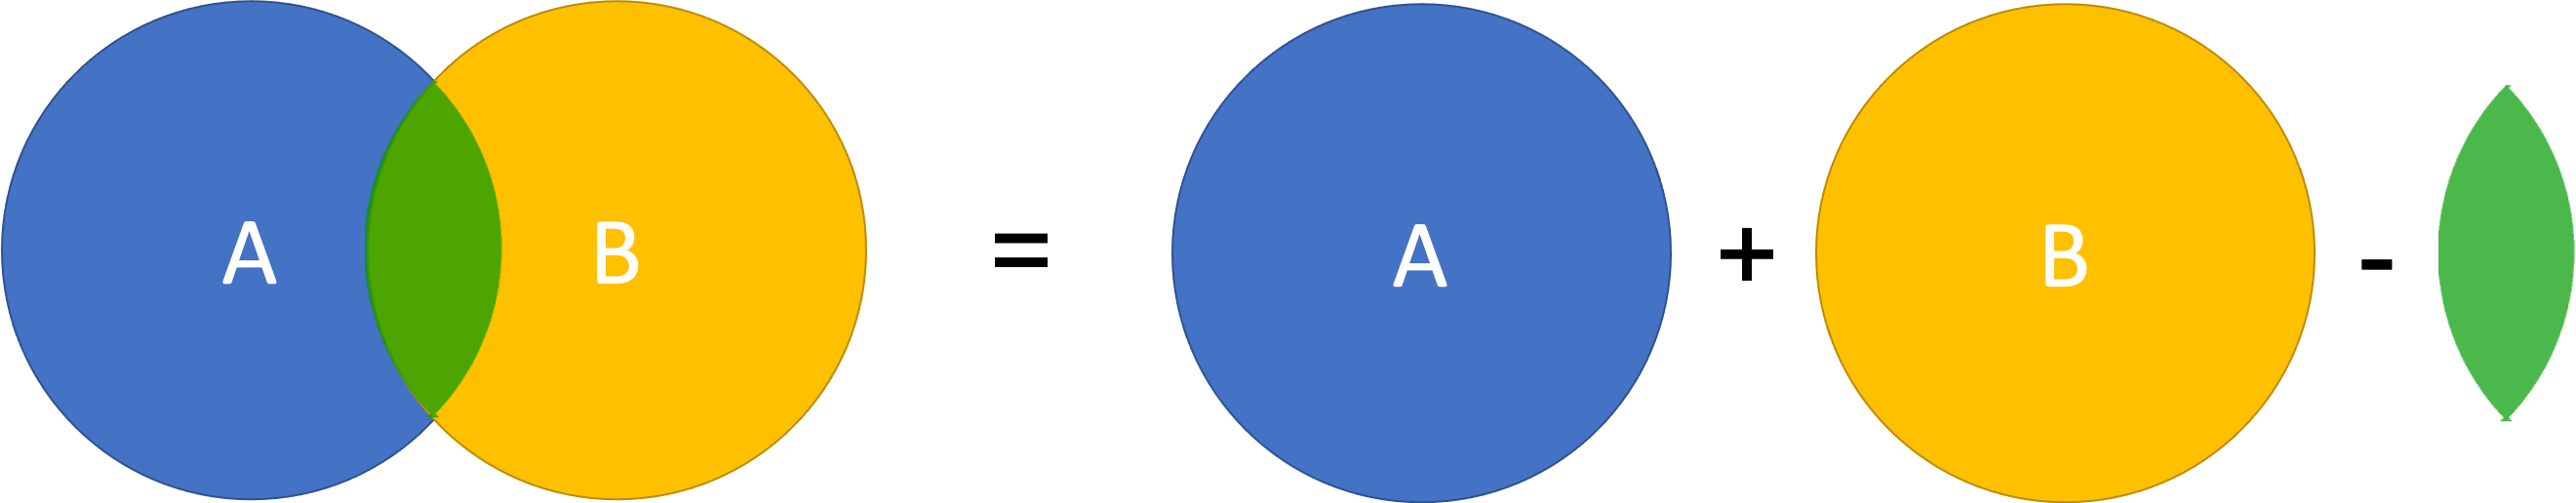
\includegraphics[width=\textwidth]{images/additive_law_of_probability_proof.png}
      \caption{A Venn-Diagram showing the proof of the additive law of probability for multiple events.}
      \label{fig:probability:multiple_events:additive}
\end{figure}

The next section presents Bayes' Theorem and it is shown how it is related to conditional probability.

\section{Bayes' Theorem}
\label{sec:probability:bayes_theorem}

Bayes' Theorem, named after Thomas Bayes, describes the probability of an event $A$, based on prior knowledge of conditions that might be related to $A$~\cite{ref:zalta:2015}. On order to derive the formal theorem and proof, first consider Definition \ref{def:probability:bayes_theorem:partition} below~\cite{ref:zalta:2015}.

\begin{definition}
      \label{def:probability:bayes_theorem:partition}
      For some positive integer, $k$, let the sets $B_{1}, B_{2}, \dots, B_{k}$ be such that

      \begin{enumerate}
            \item $S = B_{1} \cup B_{2} \cup \dots \cup B_{k}$
            \item $B_{i} \cap B_{j} = \emptyset, for i \neq j$
      \end{enumerate}

      Then the collection of sets [$B_{1}$, $B_{2}$, $\dots$, $B_{k}$] is said to be a partition of S.
\end{definition}

Bayes Theorem is then presented in Theorem \ref{th:probability:bayes_theorem:theorem} below.

\begin{theorem}[\textbf{Bayes' Theorem}]
      \label{th:probability:bayes_theorem:theorem}
      Assume that $[B_{1}, B_{2}, \dots, B_{k}]$ is a partition of $S$ such that $P(B_{i}) > 0$, for $i = 1,2, \dots, k$ then
      \begin{equation*}
            P(B_{j} \vert A) = \frac{P(A \vert B_{j})P(B_{j})}{\sum_{i=1}^{k} P(A \vert B_{i})P(B_{i})}
      \end{equation*}
\end{theorem}

\begin{proof}
      The proof follows directly from the definition of of conditional probability as was discussed in \ref{sec:probability:cond_probability}. This is shown below

      \begin{equation*}
            \begin{split}
                  P(B_{j} \vert A)
                  &= \frac{P(A \cap B_{j})}{P(A)}\\
                  &= \frac{P(A \vert B_{j})P(B_{j})}{\sum_{i=1}^{k} P(A \vert B_{i})P(B_{i})}
            \end{split}
      \end{equation*}
\end{proof}

One of the many applications of Bayes' Theorem is to do statistical inference. This is referred to as Bayesian inference. The theorem expresses how a degree of belief, expressed as a probability, should rationally change to account for the availability of related evidence.

Bayesian inference is fundamental to Bayesian statistics. Section \ref{sec:probability:bayesian_statistics} presents the detail around Bayesian statistics. However, a brief detour is required to present to the user, a number of probability distributions. These probability distributions are presented next. Consider now a number of probability distributions as they are implemented.



\section{Probability Distributions}
\label{sec:probability:probability_distributions}

Probability distributions are mathematical functions that give the probabilities of the occurrences of different possible outcomes in the experiment. They play a crucial role in the architecture and design of the \ac{BHH}. It will later be shown how the proposed \ac{BHH} makes extensive use of probability distributions and sampling to formulate its selection mechanism. The theory and equations presented in the following sections where all taken from~\citeauthor{ref:wackerly:2014}~\cite{ref:wackerly:2014}.


\subsection{Beta Distribution}
\label{sec:probability:probability_distributions:beta}

The Beta distribution is a family of univariate continuous probability distributions over some $x$, with support on the interval $[0,1]$~\cite{ref:wackerly:2014}. It is parameterised by two shape parameters $\alpha > 0$, $\alpha \in \mathbb{R}$ and $\beta > 0$, $\beta \in \mathbb{R}$. The Beta distribution is denoted as $Beta(\alpha, \beta)$. The \ac{PDF} of the Beta distribution is given below in Equation~\eqref{eq:probability:probability_distributions:beta:pdf}.

\begin{equation}
      \label{eq:probability:probability_distributions:beta:pdf}
      P(x \vert \alpha, \beta) = f_{Beta}(x; \alpha, \beta) = \frac{1}{B(\alpha, \beta)} x^{\alpha - 1} (1 - x)^{\beta - 1}
\end{equation}

where the normalising constant $B(\alpha, \beta)$ is defined below in Equation~\eqref{eq:probability:probability_distributions:beta:norm_const}.

\begin{equation}
      \label{eq:probability:probability_distributions:beta:norm_const}
      B(\alpha, \beta) = \frac{\Gamma(\alpha)\Gamma(\beta)}{\Gamma(\alpha + \beta)}
\end{equation}

and $\Gamma$ is the Gamma function as defined below in Equation~\eqref{eq:probability:probability_distributions:beta:gamma_func}.

\begin{equation}
      \label{eq:probability:probability_distributions:beta:gamma_func}
      \Gamma(n) = ( n - 1)!
\end{equation}

it should be noted that the Gamma function can also be written as shown in Equation~\eqref{eq:probability:probability_distributions:beta:gamma_func_alt} below.

\begin{equation}
      \label{eq:probability:probability_distributions:beta:gamma_func_alt}
      \Gamma(n+1) = n!
\end{equation}

It should be noted that $\alpha$ and $\beta$ determine the shape of the distribution. There exists a special case where $\alpha = \beta$. This is referred to as the \textit{symmetric} Beta distribution. In the case where $\alpha = \beta = 1$ the distribution is equivalent to the uniform distribution over all points in its support. The Beta distribution for various values of $\alpha$ and $\beta$, including the symmetric version is presented below in Figure \ref{fig:probability:probability_distributions:beta}.

\begin{figure}[htbp]
      \begin{subfigure}{0.49\textwidth}
            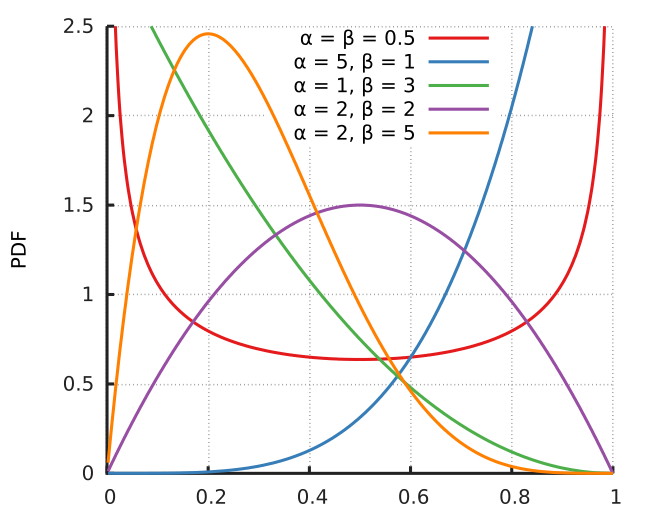
\includegraphics[width=\textwidth]{images/beta_various.png}
            \caption{Beta distribution}
            \label{fig:probability:probability_distributions:beta_normal}
      \end{subfigure}
      \begin{subfigure}{0.49\textwidth}
            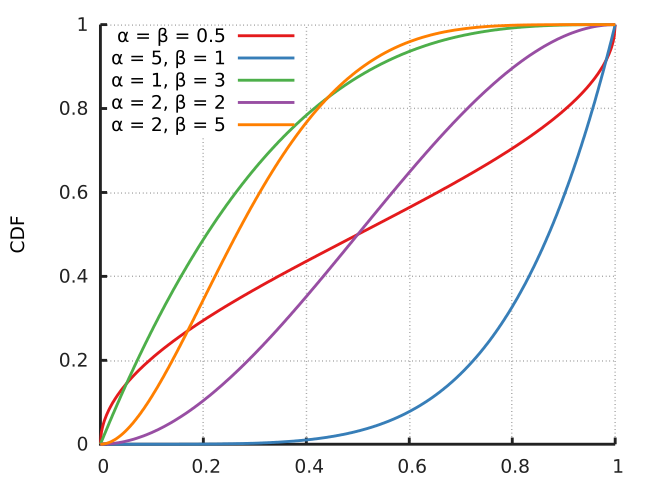
\includegraphics[width=\textwidth]{images/beta_cumulative.png}
            \caption{Cumulative Beta distribution}
            \label{fig:probability:probability_distributions:beta_cumulative}
      \end{subfigure}
      \par\bigskip
      \caption{An illustration of the Beta distribution (left)~\cite{ref:beta:2014} as well as the cumulative Beta distribution (right)~\cite{ref:cumulativebeta:2014} for various values of $\alpha$ and $\beta$ .}
      \label{fig:probability:probability_distributions:beta}
\end{figure}


The expected value of $x$ is given below in Equation~\eqref{eq:probability:probability_distributions:beta:expected_value}.

\begin{equation}
      \label{eq:probability:probability_distributions:beta:expected_value}
      E[x] = \frac{\alpha}{\alpha + \beta}
\end{equation}

Similarly, the expected value of the natural logarithm of $x$ can be calculated as shown below in Equation~\eqref{eq:probability:probability_distributions:beta:expected_value_ln}.

\begin{equation}
      \label{eq:probability:probability_distributions:beta:expected_value_ln}
      E[\ln(x)] = \psi({\alpha}) - \psi(\alpha + \beta)
\end{equation}

where $\psi$ is the logarithmic derivative of the Gamma function, called the \textit{Digamma} function. The Digamma function is given below in Equation~\eqref{eq:probability:probability_distributions:beta:digamma}.

\begin{equation}
      \label{eq:probability:probability_distributions:beta:digamma}
      \psi(n) = \frac{d}{dn}\ln(\Gamma(n)) = \frac{\Gamma'(n)}{\Gamma(n)}
\end{equation}

Finally, the mode of the distribution is given in Equation~\eqref{eq:probability:probability_distributions:beta:mode} below.

\begin{equation}
      \label{eq:probability:probability_distributions:beta:mode}
      M[x] = E[x] - 1 = \frac{\alpha - 1}{\alpha + \beta - 1}
\end{equation}










\subsection{Dirichlet Distribution}
\label{sec:probability:probability_distributions:dirichlet}


The Dirichlet distribution is a family of multivariate continuous probability distributions over some $x$ in $K$ dimensions ~\cite{ref:wackerly:2014}. The Dirichlet distribution is the multivariate generalization of the Beta distribution and is thus sometimes referred to by its alternative name, the Multivariate Beta Distribution. The Dirichlet distribution is parameterised by some vector $\alpha = (\alpha_{1}$,  $\dots, \alpha_{K})$ $\forall_{k=1}^{K} \alpha_{k} > 0$, $\alpha_{k} \in \mathbb{R}$. $\alpha$ is referred to as the concentration parameter. It is later shown in Chapter \ref{chap:bhh} that this parameter plays a vital role in the optimisation process of the \ac{BHH}. The Dirichlet distribution of order $K \geq 2$ with parameters $\alpha$, denoted $Dir(\alpha)$, has a \ac{PDF} as given in Equation~\eqref{eq:probability:probability_distributions:dirichlet:pdf} below.

\begin{equation}
      \label{eq:probability:probability_distributions:dirichlet:pdf}
      P(x \vert \alpha) =  f_{Dir}(x; K, \alpha) = \frac{1}{B(\alpha)}  \prod_{k=1}^{K} x_{k}^{\alpha_{k} - 1}
\end{equation}

where the normalising constant $B(\alpha)$ is defined in Equation~\eqref{eq:probability:probability_distributions:dirichlet:norm_cost}.

\begin{equation}
      \label{eq:probability:probability_distributions:dirichlet:norm_cost}
      B(\alpha) = \frac{\prod_{k=1}^{K} \Gamma(\alpha_{k})}{\Gamma(\alpha_{0})}
\end{equation}

and $\alpha_{0}$ is defined in Equation~\eqref{eq:probability:probability_distributions:dirichlet:alpha_0} below.

\begin{equation}
      \label{eq:probability:probability_distributions:dirichlet:alpha_0}
      \alpha_{0} = \sum_{k=1}^{K}\alpha_{k}
\end{equation}

Importantly, the set $\{x_{k}\}_{k=1}^{K}$ belongs to the standard $K-1$ probability simplex $S$, meaning that $x_{K} = 1 - \sum_{k=1}^{K-1}x_{k}$ with support $\forall_{k=1}^{K} x \in [0,1]$. Under the simplex $S$, this means that the sum over all values of the vector $x$ must be 1. The simplex can thus be rewritten as $\sum_{k=1}^{K}x_{k} = 1$.

Similar to the Beta distribution, $\alpha$ determines the shape of the distribution in $K$ dimensions and thus, there also exist a special case, referred to as the \textit{symmetric} distribution when $\forall_{k=1}^{K} \alpha_{k} = c$, where $c$ is some constant. In the case where $c = 1$, the distribution is referred to as a \textit{flat} distribution and yields the uniform distribution over all points in $S$. The Dirichlet distribution of order $K = 3$, for various values of $\alpha$, including the symmetric version is presented in Figure \ref{fig:probability:probability_distributions:dirichlet} below.

\begin{figure}[htbp]
      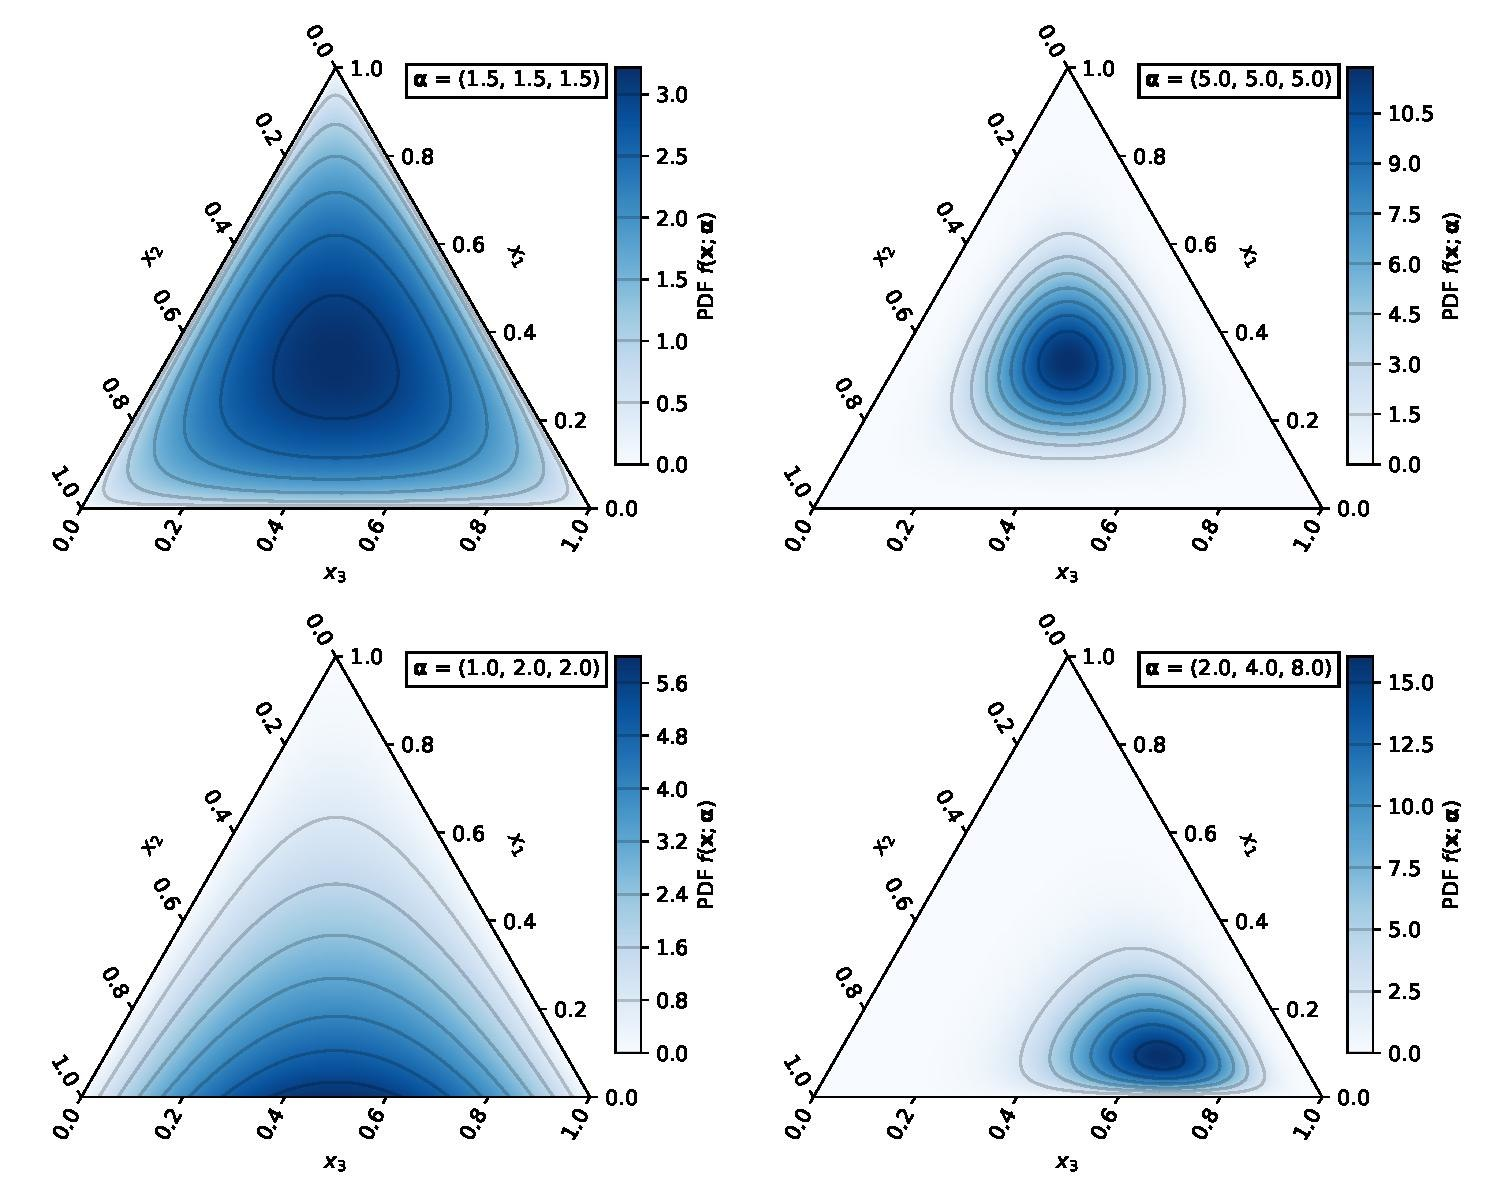
\includegraphics[width=\textwidth]{images/dirichlet.jpg}
      \caption{The \acp{PDF} for the Dirichlet distribution over the 2-simplex. The concentration parameter $\alpha$ is varied. The values of $\alpha$ are set to (1.5, 1.5, 1.5), (5, 5, 5), (1, 2, 2), and (2, 4, 8) respectively, read from top to bottom, left to right. The values of the \ac{PDF} are shown by the color maps with contour lines at equal values as indicated in the color bars~\cite{ref:dirichlet:2020}.}
      \label{fig:probability:probability_distributions:dirichlet}
\end{figure}

The expected value of $x$ can be calculated as shown in Equation~\eqref{eq:probability:probability_distributions:dirichlet:expected_value} below.

\begin{equation}
      \label{eq:probability:probability_distributions:dirichlet:expected_value}
      E[x_{k}] = \frac{\alpha_{k}}{\alpha_{0}}
\end{equation}

Similarly, the expected value of the natural logarithm of $x_{k}$ can be calculated as defined in Equation~\eqref{eq:probability:probability_distributions:dirichlet:expected_value_ln} below.

\begin{equation}
      \label{eq:probability:probability_distributions:dirichlet:expected_value_ln}
      E[\ln(x_{k})] = \psi({\alpha_{k}}) - \psi(\alpha_{0})
\end{equation}

where $\psi$ is the Digamma function as defined in Equation~\eqref{eq:probability:probability_distributions:beta:digamma}. Finally, the mode of the distribution is given in Equation~\eqref{eq:probability:probability_distributions:dirichlet:mode} below.

\begin{equation}
      \label{eq:probability:probability_distributions:dirichlet:mode}
      \begin{split}
            M[x_{k}] &= E[{x_{k}] -K^{-1}} \\
            &=  \frac{\alpha_{k} - 1}{\alpha_{0} - K}
      \end{split}
\end{equation}


\subsection{Bernoulli Distribution}
\label{sec:probability:probability_distributions:bernoulli}

The Bernoulli distribution is a discrete probability distribution over some random variable $x$ that takes the value of $1$ with probability $\theta$ and $0$ with probability $1-\theta$ ~\cite{ref:wackerly:2014}. It is denoted as $Ber(\theta)$ with support $x \in \{0, 1\}$. In probability theory, the Bernoulli distribution is often used to explain the possible outcomes of a single experiment that asks a \textit{yes-no} question such as flipping a coin. The outcome of such an experiment is a boolean value. The Bernoulli distribution has a \ac{PMF} as given below in Equation~\eqref{eq:probability:probability_distributions:bernoulli:pmf}.

\begin{equation}
      \label{eq:probability:probability_distributions:bernoulli:pmf}
      P(x \vert \theta) = f_{Ber}(x; \theta) =
      \begin{cases}
            \theta     & \text{if}\ x=1 \\
            1 - \theta & \text{if}\ x=0
      \end{cases}
\end{equation}

The above equation can also be expressed as show in Equation~\eqref{eq:probability:probability_distributions:bernoulli:alt} below.

\begin{equation}
      \label{eq:probability:probability_distributions:bernoulli:alt}
      f_{Ber}(x; \theta) = \theta^{x}(1-\theta)^{1-x}
\end{equation}

The mean of the Bernoulli distribution approaches $\theta$ over many samples according to the \ac{CLT}~\cite{ref:grinstead:1997}. Figure \ref{fig:probability:probability_distributions:bernoulli:coin} shows a simulation of a fair-coin flipping simulation. One can see how the mean converges to 0.5 for various sample sizes.

\begin{figure}[htbp]
      \begin{subfigure}{0.49\textwidth}
            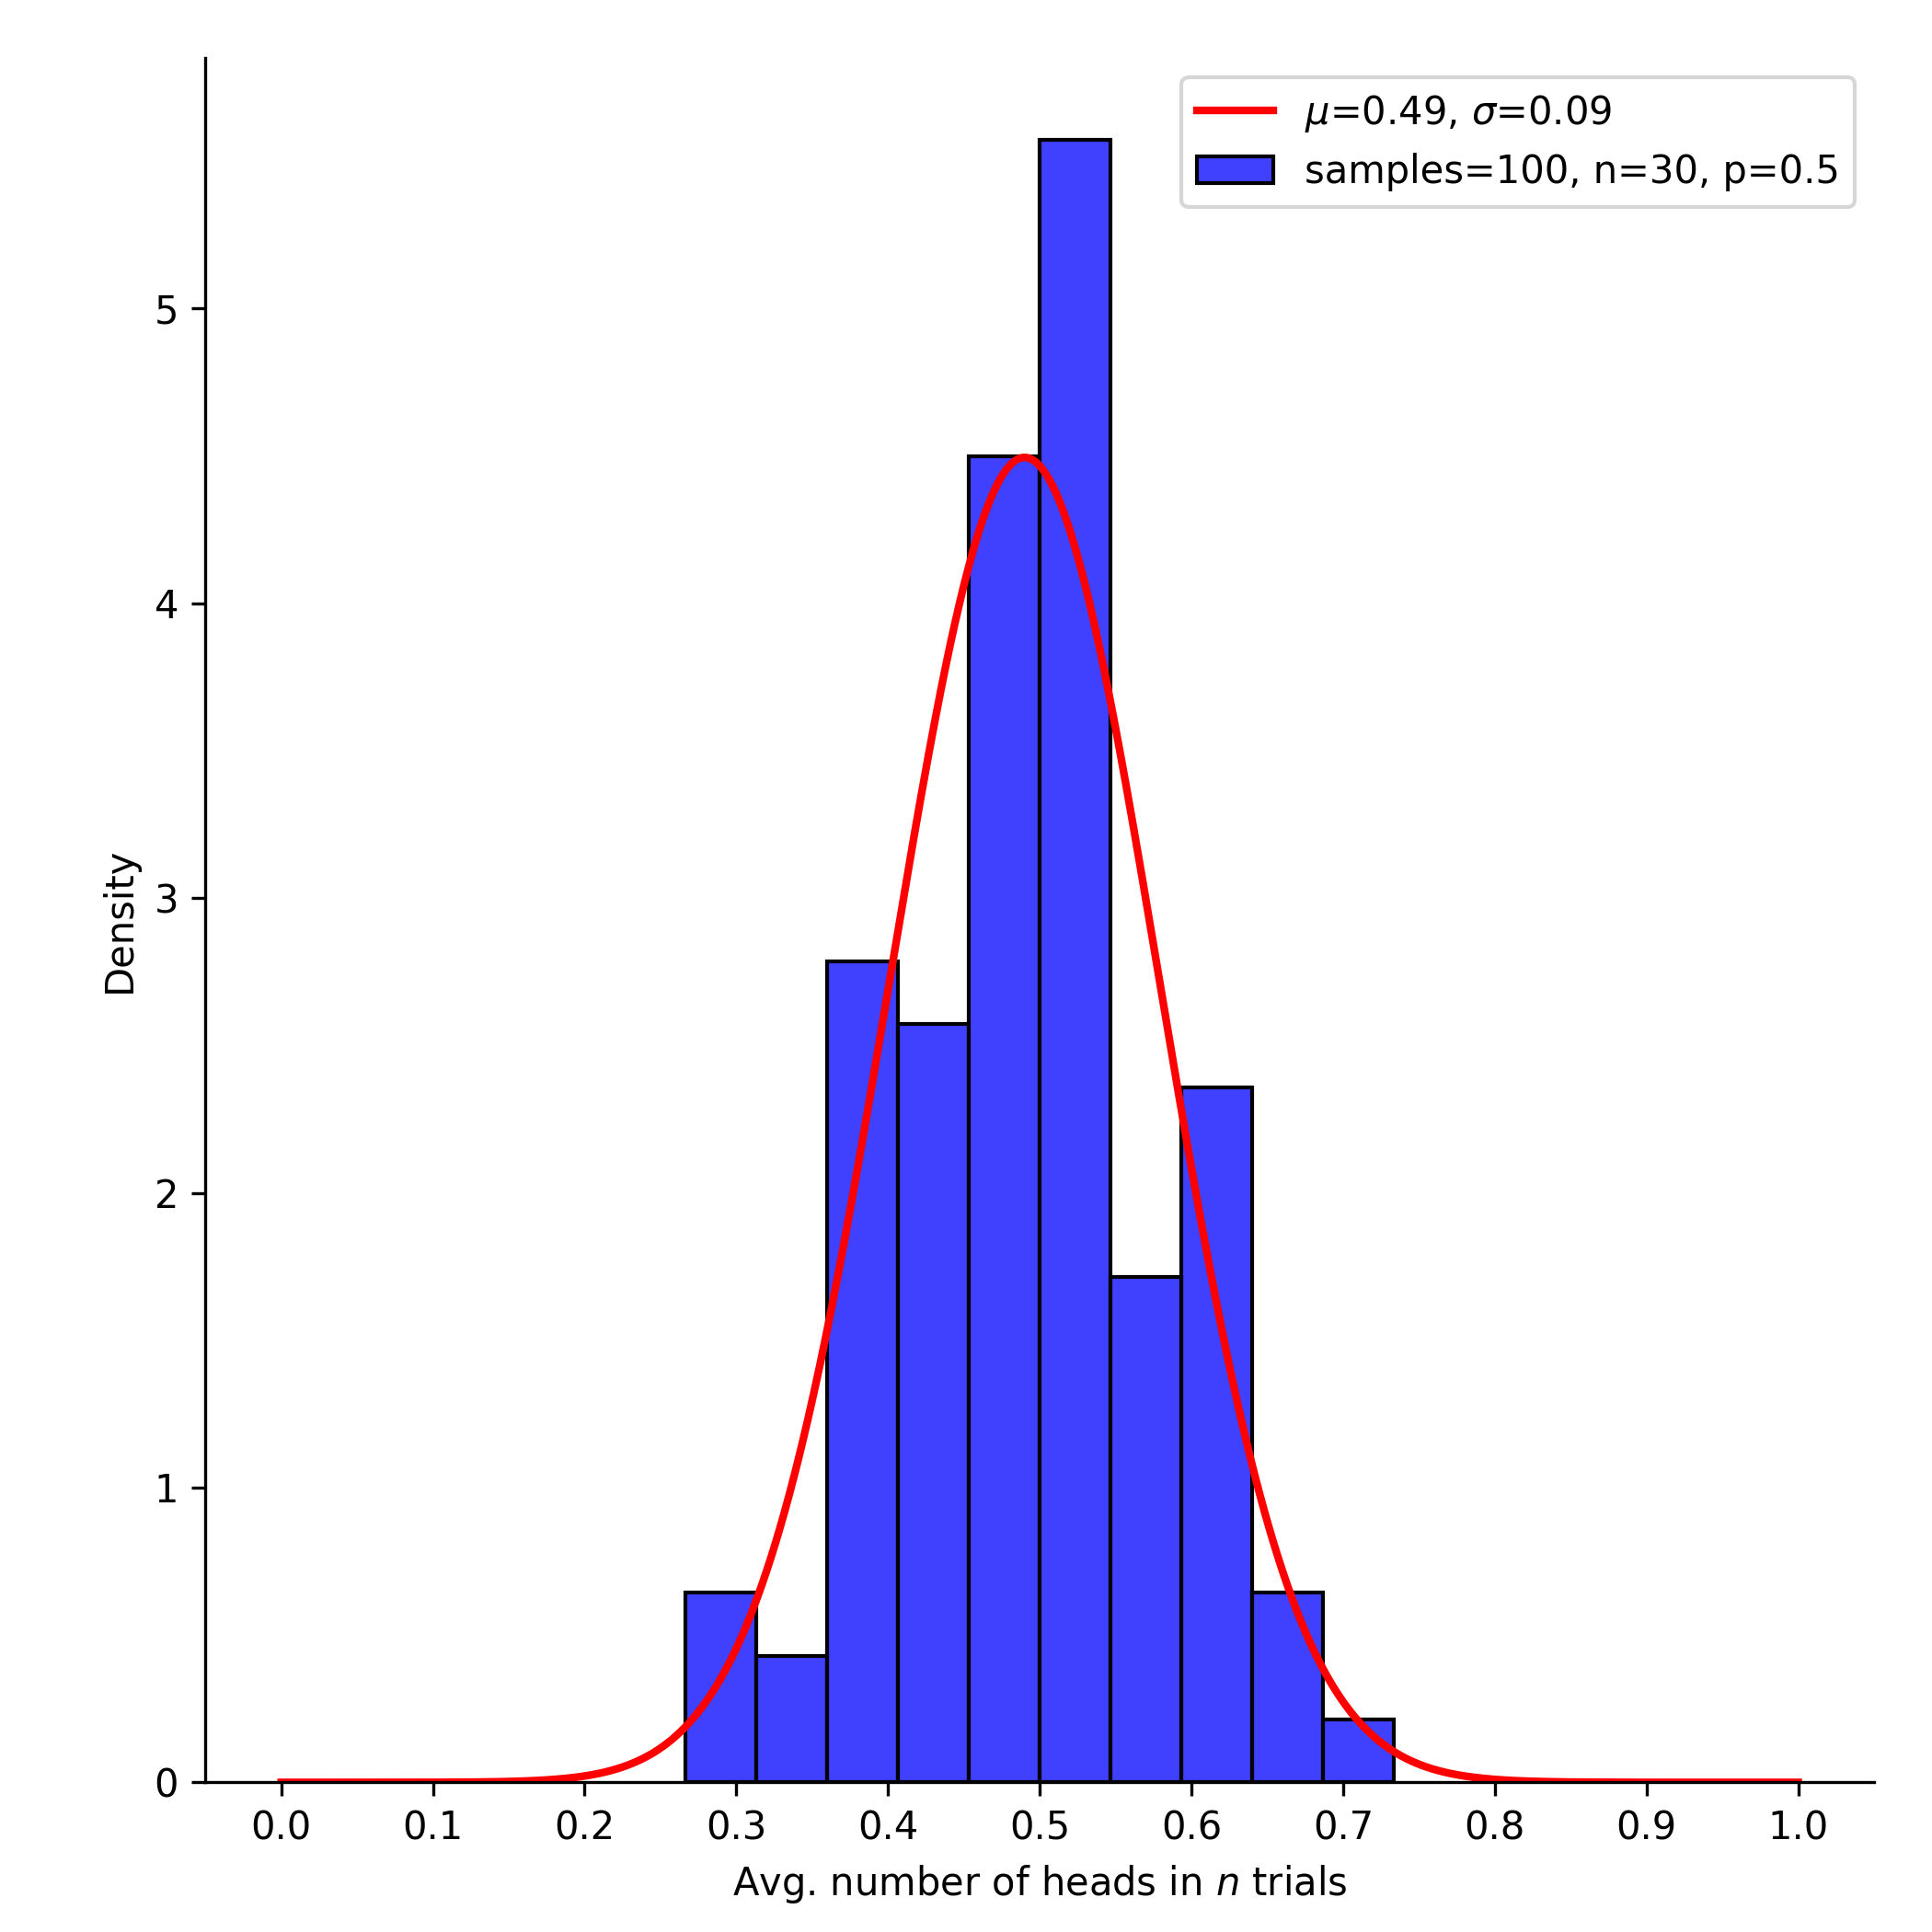
\includegraphics[width=\textwidth]{images/coin_flip_samples_100.png}
            \caption{100 Samples}
            \label{fig:probability:probability_distributions:bernoulli:coin_100}
      \end{subfigure}
      \begin{subfigure}{0.49\textwidth}
            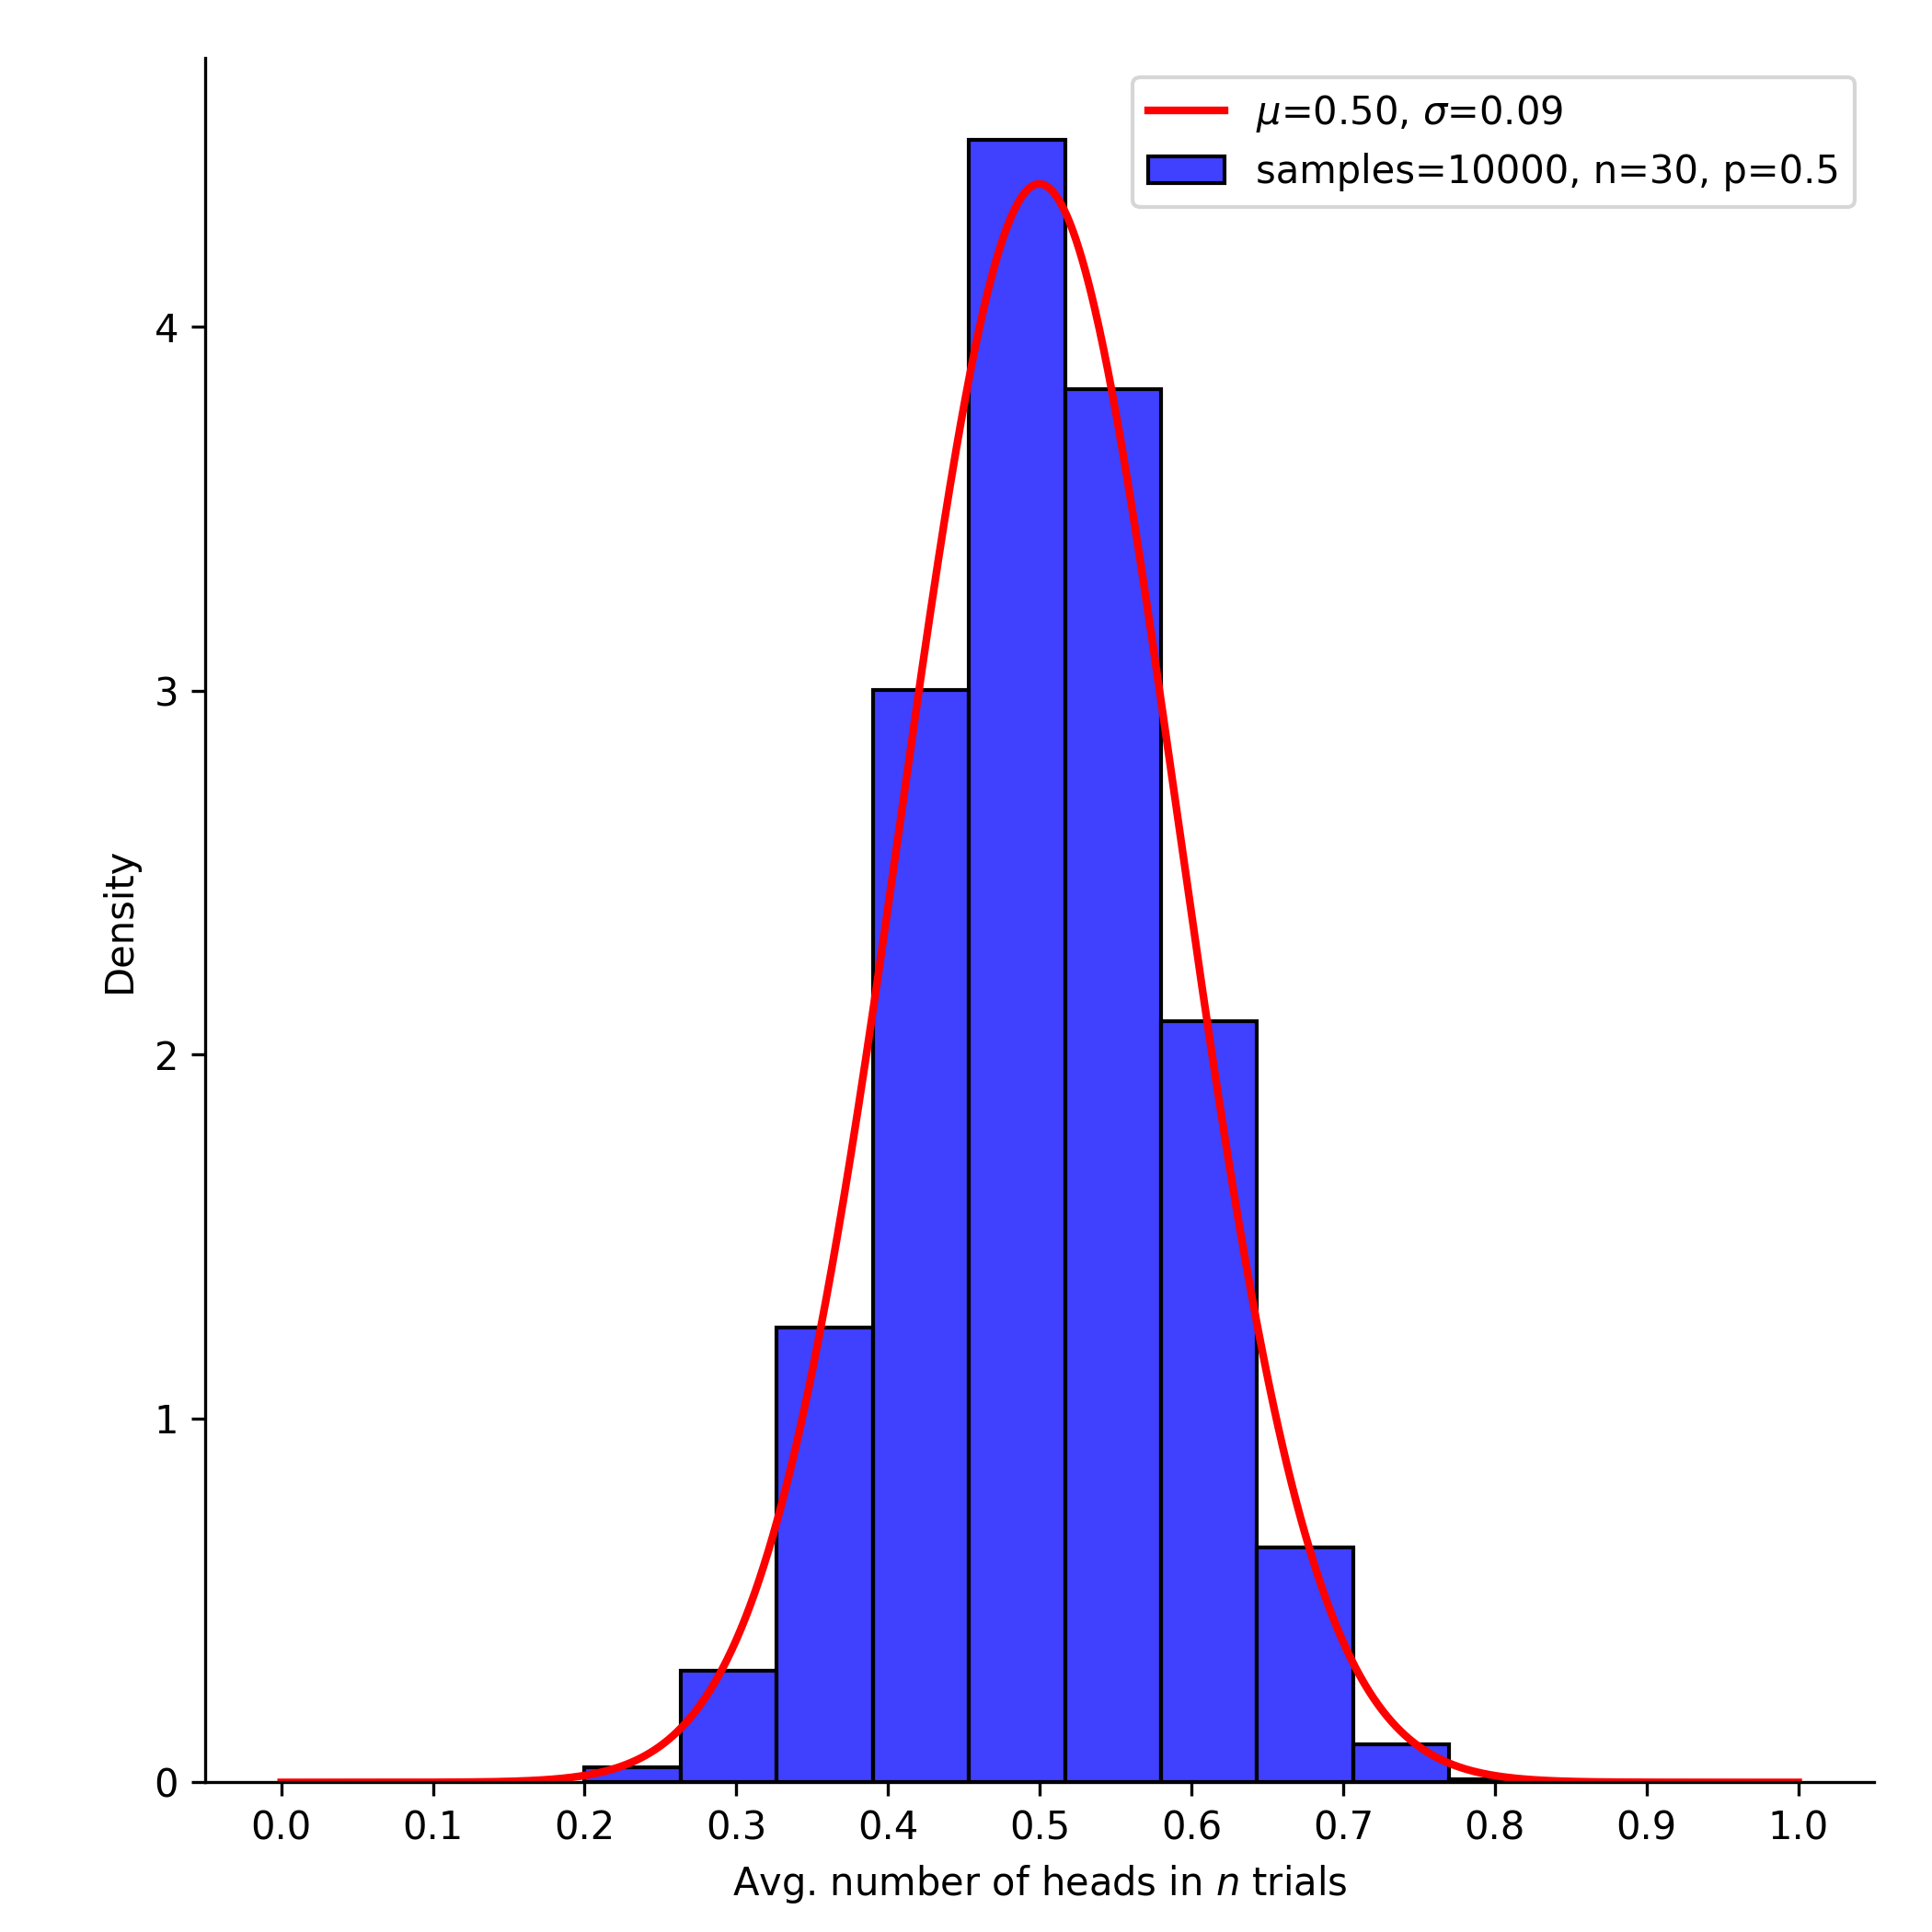
\includegraphics[width=\textwidth]{images/coin_flip_samples_10000.png}
            \caption{1000 Samples}
            \label{fig:probability:probability_distributions:bernoulli:coin_1000}
      \end{subfigure}
      \par\bigskip
      \caption{An illustration of the the coin flip situation for different sample sizes that show the convergence of the mean as per the \ac{CLT}.}
      \label{fig:probability:probability_distributions:bernoulli:coin}
\end{figure}

The expected value of the distribution is thus given according to Equation~\eqref{eq:probability:probability_distributions:bernoulli:expected_value} below.

\begin{equation}
      \label{eq:probability:probability_distributions:bernoulli:expected_value}
      E[x] = \theta
\end{equation}

while the mode of the distribution is given in Equation~\eqref{eq:probability:probability_distributions:bernoulli:mode} below.

\begin{equation}
      \label{eq:probability:probability_distributions:bernoulli:mode}
      M[x_{k}] =
      \begin{cases}
            0   & \text{if}\ \theta < 0.5 \\
            0,1 & \text{if}\ \theta = 0.5 \\
            1   & \text{if}\ \theta > 0.5 \\
      \end{cases}
\end{equation}




\subsection{Binomial Distribution}
\label{sec:probability:probability_distributions:bin}


The Binomial distribution is a discrete probability distribution over a random variable $x$ taking on a number of successes in $N$ sequential independent experiments that each ask a \textit{yes-no} question~\cite{ref:wackerly:2014}. The probability of a single independent experiment yielding a success is given as $\theta$ and the Binomial distribution is denoted as $Bin(N, \theta)$ with support $x \in \{0, 1, \dots, N\}$.  It should be noted that the Binomial distribution is the extension of the Bernoulli distribution over $N$ independent sequential experiments and thus, each experiment also yields some boolean outcome. When $N=1$, the experiment is referred to as a Bernoulli trial and the distribution is just a Bernoulli distribution. When $N > 1$, the sequence of outcomes is referred to as a Bernoulli process. The \ac{PMF} of the Binomial distribution is given in Equation~\eqref{eq:probability:probability_distributions:binomial:pmf} below.

\begin{equation}
      \label{eq:probability:probability_distributions:binomial:pmf}
      P(x \vert \theta; N) = f_{Bin}(x; N, \theta) = \binom{N}{x} \theta^{x}(1-\theta)^{1-x}
\end{equation}

Similar to the Bernoulli distribution, the mean of the Binomial distribution is $N\theta$ given the \ac{CLT} as was shown in Figure \ref{fig:probability:probability_distributions:bernoulli:coin}. The expected value of the Binomial distribution is thus given in Equation~\eqref{eq:probability:probability_distributions:binomial:expected_value} below.

\begin{equation}
      \label{eq:probability:probability_distributions:binomial:expected_value}
      E[x] = N\theta
\end{equation}

The mode of the distribution is given in Equation~\eqref{eq:probability:probability_distributions:binomial:mode} below.

\begin{align}
      \label{eq:probability:probability_distributions:binomial:mode}
      \begin{split}
            M[x_{k}] &= E[x] + \theta \\
            &= N\theta  + \theta \\
            &= (N  + 1)\theta
      \end{split}
\end{align}



\subsection{Categorical Distribution}
\label{sec:probability:probability_distributions:categorical}

The Categorical distribution is a discrete probability distribution over some random variable $x$, taking on any one of $K$ possible categories~\cite{ref:wackerly:2014}. There is no innate underlying ordering to these categories and therefore, for simplicity, each category is assigned a numerical representative value such that $k = (1, \dots, K)$. The probabilities for all outcomes is given by the probability vector $\theta = (\theta_{1}, \dots, \theta_{K})$.  This means that the probability $P(x=k)=\theta_{k}$ has support $x \in \{1, \dots, K\}$. The Categorical distribution, denoted $Cat(\theta)$ is the generalization of the Bernoulli distribution and is sometimes referred to it by its alternative names, the generalised Bernoulli Distribution or the Multinoulli distribution. In probability theory, the Categorical distribution is often used to explain the outcome of a single experiment with more than two possible outcomes such as rolling a die~\cite{ref:wackerly:2014}. The \ac{PMF} of the Categorical distribution is given in Equation~\eqref{eq:probability:probability_distributions:categorical:pmf} below.

\begin{equation}
      \label{eq:probability:probability_distributions:categorical:pmf}
      P(x \vert \theta; K) = f_{Cat}(x; K, \theta) = \prod_{k=1}^{K}\theta_{k}^{[x = k]}
\end{equation}

where $[x = k]$ is the Iversion Bracket~\cite{ref:iverson:1962}, yielding 1 if $x = k$ and 0 otherwise. From this, one can conclude that for a given class $k$, the categorical distribution simply yields $\theta_{k}$ as is shown in Equation~\eqref{eq:probability:probability_distributions:categorical:pmf_k} below.

\begin{equation}
      \label{eq:probability:probability_distributions:categorical:pmf_k}
      f_{Cat}(x=k; K, \theta) = \theta_{k}
\end{equation}

The random variable $x$ can also be encoded in binary format, yielding a vector $x = (x_{1}, \dots, x_{K})$ of Bernoulli distributions such that the support is $\forall_{k=1}^{K} x_{k} \in \{0, 1\}$. Importantly, if the outcome of the random event is of category $k$, then $x_{k} = 1$ and $\forall_{j=1}^{K} x_{j} = 0, j \neq k$ so that the standard $K-1$ probability simplex $S$ still holds. The \ac{PMF} of the Categorical distribution can then be rewritten as follows in Equation~\eqref{eq:probability:probability_distributions:categorical:pmf_alt} below.

\begin{equation}
      \label{eq:probability:probability_distributions:categorical:pmf_alt}
      f_{Cat}(x; K, \theta) = \prod_{k=1}^{K}\theta_{k}^{\mathbbm{1}_{1}(x_{k})}
\end{equation}

where $\mathbbm{1}(x_{k})$ is the \textit{indicator function}, yielding 1 if $x_{k} = 1$ and 0 otherwise.

Since there is no innate order to the underlying categories, the mean of the distribution does not yield any relevant information. The mode of the distribution is given in Equation~\eqref{eq:probability:probability_distributions:categorical:mode} below.

\begin{equation}
      \label{eq:probability:probability_distributions:categorical:mode}
      M[x] = \argmax_{k}(\theta_{1}, \dots, \theta_{K})
\end{equation}


\subsection{Multinomial Distribution}
\label{sec:probability:probability_distributions:multinomial}

The Multinomial distribution is a discrete probability distribution over some random variable $x = (x_{1}, \dots\, x_{K})$ that takes on the counts for each occurrence of $K$ possible classes in $N$ independent trials~\cite{ref:wackerly:2014}. The probabilities for all possible outcomes in a single trial is given by the probability vector $\theta = (\theta_{1}, \dots, \theta_{K})$. The Multinomial distribution, denoted $Mul(N, K, \theta)$, is thus the generalization of the Binomial distribution to $K$ dimensions. Consider the following special cases.

\begin{itemize}
      \item When $K$ is 2 and $N = 1$, the Multinomial distribution is the Bernoulli distribution.
      \item When $K$ is 2 and $N > 1$, the Multinomial distribution is the Binomial distribution.
      \item When $K > 2$ and $N = 1$, the Multinomial distribution is the Categorical distribution.
\end{itemize}

The support for the Multinomial is $\forall_{i=1}^{K} x_{k} \in \{1, \dots, N\}, \sum_{k=1}^{K}x_{k} = N$ and the \ac{PMF} for the Multinomial distribution is given below in Equation~\eqref{eq:probability:probability_distributions:multinomial:pmf}.

\begin{equation}
      \label{eq:probability:probability_distributions:multinomial:pmf}
      P(x \vert \theta; N; K) = f_{Mul}(x; N, K, \theta) = \frac{N!}{\prod_{k=1}^{K}x_{k}!} \prod_{k=1}^{K}\theta_{k}^{x_{k}}
\end{equation}

Similar to the Categorical distribution, the random variable $x$ can also be encoded in binary format, yielding an $N \times K$ matrix $X$ of Bernoulli distributions. The support is then given as $X \in \{0, 1\}^{N \times K}, \forall_{i=1}^{N}\sum_{k=1}^{K} x_{i,k} = 1$ so that the standard $K-1$ probability simplex $S$ still holds for each trial. The \ac{PMF} of the Multinomial distribution can then be rewritten as is presented in Equation~\eqref{eq:probability:probability_distributions:multinomial:pmf_alt}

\begin{equation}
      \label{eq:probability:probability_distributions:multinomial:pmf_alt}
      \begin{split}
            f_{Mul}(x; N, K, \theta) &= \frac{N!}{\prod_{k=1}(\sum_{i=1}^{N}x_{i, k})!}\prod_{i=1}^{N}\prod_{k=1}^{K}\theta_{k}^{\mathbbm{1}_{1}(x_{i,k})} \\
            &= \frac{N!}{\prod_{k=1}(\sum_{i=1}^{N}x_{i, k})!} \prod_{k=1}^{K}\theta_{k}^{\sum_{i=1}^{N}\mathbbm{1}_{1}(x_{i,k})} \\
            &= \frac{N!}{\prod_{k=1}(\sum_{i=1}^{N}x_{i, k})!} \prod_{k=1}^{K}\theta_{k}^{N_{k}} \\
      \end{split}
\end{equation}

where $N_{k}$ is a summary variable denoting the number of times a category $k$ occurs over all trials in $N$.

The reason why the Categorical and Multinomial distributions are presented as binary encoded vectors is to simplify the proof of their conjugate priors as will be shown next. This is further supported by the fact that \acp{NN} often use binary encoding of feature vectors. The combination of these probabilistic methods and \acp{NN} forms the basic of this dissertation.


\section{Conjugate Priors}
\label{sec:probability:conjugate_priors}

\citeauthor{ref:wackerly:2014}\cite{ref:wackerly:2014} states that conjugate priors are prior probability distributions that results in posterior distributions that are of the same functional form $\mathcal{A}(v)$ as the prior, but with different parameter values. This section considers the conjugate priors for the Binomial likelihood and Categorical/Multinomial likelihood. Each of these are presented next.

\subsection{Binomial Likelihood}
\label{sec:probability:conjugate_priors:binom_likelihood}

The conjugate prior to a Bernoulli distribution is the Beta distribution
\cite{ref:wackerly:2014}. This is shown by demonstrating that the posterior distribution has the
same functional form $\mathcal{A}(v)$ as the prior distribution as follows. \\\\
\textbf{Setup}:

\begin{itemize}
      \item Let $I$ be a number of independent, identical  (iid) random events.

      \item Let $\alpha \in \mathbb{R}, \alpha > 0$ and $\beta \in \mathbb{R}, \beta >0$ be the shape parameters to the Beta distribution.

      \item Let $\theta$ be the probability of a success. With $\theta | \alpha, \beta \sim Beta(\alpha, \beta)$.

      \item $P(\theta)$ is the prior probability distribution with the functional form $\mathcal{A}(v)$.

      \item Let $X = (x_{1}, \dots, x_{I})$ be the outcomes of independent, identical random events, each with boolean outcome. That is $x_{i} | \theta \overset{\text{iid}}{\sim} Ber(\theta)$ and thus $\mathcal{L}(x_{i} \vert \theta)$ is the Bernoulli likelihood.

      \item Let $\mathcal{D}$ denote all the prior data $X$, parameterised by $\alpha$, $\beta$.

      \item Let $N_{1} = \sum_{i=1}^{I} \mathbbm{1}(x_{i} = 1)$ and $N_{0} = \sum_{i=1}^{I} \mathbbm{1}(x_{i} = 0)$.
\end{itemize}

The Bernoulli likelihood is then given in Equation~\eqref{eq:probability:conjugate_priors:binom_likelihood:likelihood} below.

\begin{equation}
      \label{eq:probability:conjugate_priors:binom_likelihood:likelihood}
      \begin{split}
            \mathcal{L}(\mathcal{D}) &=  P(\mathcal{D} | \theta) \\
            &\propto \theta^{N_{1}}(1-\theta)^{N_{0}}
      \end{split}
\end{equation}

By Bayes Theorem, the posterior distribution with given prior data $\mathcal{D}$ is given in Equation~\eqref{eq:probability:conjugate_priors:binom_likelihood:posterior} below.

\begin{equation}
      \begin{split}
            \label{eq:probability:conjugate_priors:binom_likelihood:posterior}
            P(\theta \vert \mathcal{D}) &= \frac{P(\mathcal{D} | \theta) P(\theta)}{P(\mathcal{D})}
      \end{split}
\end{equation}

Since the denominator sums to $1$, one could get rid of the denominator and constants for the Bernoulli likelihood and the Beta prior, by expressing the posterior as proportional to the likelihood times the prior as is shown in Equation~\eqref{eq:probability:conjugate_priors:binom_likelihood:posterior_propto} below.

\begin{equation}
      \label{eq:probability:conjugate_priors:binom_likelihood:posterior_propto}
      \begin{split}
            P(\theta | \mathcal{D}) &\propto \left[\theta^{N_{1}}(1-\theta)^{N_{0}}\right] \left[\theta^{\alpha - 1} (1 - \theta)^{\beta - 1}\right] \\
            &\propto \theta^{(N_{1} + \alpha) - 1}(1-\theta)^{(N_{0} + \beta) - 1} \\
            &\propto Beta(N_{1} + \alpha, N_{0} + \beta)
      \end{split}
\end{equation}

It is show that the posterior distribution is of the same functional form $\mathcal{A}(v)$ as the prior, but with updated prior parameters $\alpha' = N_{1} + \alpha$ and $\beta' = N_{0} + \beta$. This shows that the Beta distribution is the conjugate prior to the Bernoulli likelihood.


\subsection{Categorical and Multinomial Likelihood}
\label{sec:probability:conjugate_priors:cat_mult_likelihood}

The conjugate prior to a Categorical and Multinomail distribution is the Dirichlet distribution~\cite{ref:wackerly:2014}. Similar to the proof of the conjugate prior for the Bernoulli distribution as shown in Section \ref{eq:probability:conjugate_priors:binom_likelihood:posterior} above, this means that the posterior distribution must have the same functional form $\mathcal{A}(v)$ as the prior distribution. This is shown as follows. \\\\
\textbf{Setup}:

\begin{itemize}
      \item Let $I$ be a number of independent, identical (iid) random events.

      \item Let $K$ be a number of possible outcomes for each event, with $K \geq 2$.

      \item Let $\alpha = (\alpha_{1}, \dots, \alpha_{K}), \forall_{k=1}^{K} \alpha_{k} \in \mathbb{R}, \alpha_{k} > 0$ be the concentration parameters to the Dirichlet distribution.

      \item Let $\theta = (\theta_{1}, \dots, \theta_{K}), \forall_{k=1}^{K} \theta{k} \in (0,1), \sum_{k}^{K} \theta{k} = 1$ be the probability of each class in $K$ and $\theta$ belongs to the standard $K-1$ probability simplex $S$. With $\theta | \alpha \sim Dir(K, \alpha)$.

      \item $P(\theta)$ is the prior probability distribution with the functional form $\mathcal{A}(v)$.

      \item Let $X = (x_{1}, \dots, x_{I})$ be the outcomes of independent, identical random events, each with $K$ possible outcomes. That is $x_{i} | \theta \overset{\text{iid}}{\sim} Cat(\theta)$ and thus $\mathcal{L}(x_{i} \vert \theta)$ is the Categorical likelihood.

      \item Let $\mathcal{D}$ denote all the prior data $X$, parameterised by $\alpha$.

      \item Let $N = (N_{1}, \dots, N_{K}), N_{k} = \sum_{i=1}^{I} \mathbbm{1}(x_{i,k} = 1)$, denote the counts for each occurrence of a class $k$.
\end{itemize}

The likelihood of the Categorical and Multinomial distributions is then given in Equation~\eqref{eq:probability:conjugate_priors:mult_likelihood:likelihood} below.

\begin{equation}
      \label{eq:probability:conjugate_priors:mult_likelihood:likelihood}
      \begin{split}
            \mathcal{L}(\mathcal{D}) &=  P(\mathcal{D} | \theta) \\
            &\propto \prod_{k=1}^{K} \theta_{k}^{N_{k}}
      \end{split}
\end{equation}

By Bayes Theorem, the posterior distribution with given prior data $\mathcal{D}$ is given in Equation~\eqref{eq:probability:conjugate_priors:mult_likelihood:posterior} below.

\begin{equation}
      \label{eq:probability:conjugate_priors:mult_likelihood:posterior}
      \begin{split}
            P(\theta \vert \mathcal{D}) &= \frac{P(\mathcal{D} \vert \theta) P(\theta)}{P(\mathcal{D})}
      \end{split}
\end{equation}

Since the denominator sums to $1$, one could get rid of the denominator and constants for the Dirichlet prior,by expressing the posterior as proportional to the likelihood times the prior as is shown in Equation~\eqref{eq:probability:conjugate_priors:mult_likelihood:posterior_propto} below.

\begin{equation}
      \label{eq:probability:conjugate_priors:mult_likelihood:posterior_propto}
      \begin{split}
            P(\theta \vert \mathcal{D}) &\propto \prod_{k=1}^{K} \theta_{k}^{N_{k}} \prod_{k=1}^{K} \theta_{k}^{\alpha_{k} - 1}\\
            &\propto \prod_{k=1}^{K} \theta_{k}^{(N_{k} + \alpha_{k}) - 1} \\
            &\propto Dir(K, N + \alpha)
      \end{split}
\end{equation}

Is it shown that the posterior distribution is of the same form $\mathcal{A}(v)$ as the prior, but with updated prior parameters $\alpha' = N + \alpha$. This shows that the Dirichlet distribution is the conjugate prior to the Categorical and Multinomial likelihood.

The next section aims to provide the reader with the concept of Bayesian statistics and it is shown how Bayesian inference and Bayesian analysis can be used to to train a \ac{HH}.


\section{Bayesian Statistics}
\label{sec:probability:bayesian_statistics}

In general, there are two main views to probability and statistics. These include the \textit{frequentist} and the \textit{Bayesian} view of statistics. Naturally, Bayesian statistics is based on Bayes' Theorem as was presented in Section \ref{sec:probability:bayes_theorem}. Bayesian statistics describe the probability of an event in terms of some belief based on previous knowledge of the event and the conditions under which the event happens~\cite{ref:hackenberger:2019}. To introduce the concept of Bayesian inference and analysis, one first need to understand the difference between these two approaches. Bayesian statistics out-date the frequentist approach, but lacked interest in the early days partly because of the limited applications where the conjugate priors where known~\cite{ref:hackenberger:2019}. More recent advancements in mathematical methods popularised the Bayesian approach again. A notable contribution to this switch was the invention of \ac{MCMC} in the 1950's. This family of algorithms allowed for the construction of random sampling algorithms from a probability distribution which allows for the calculation of Bayesian hierarchical models~\cite{ref:hackenberger:2019}. Soon after followed one of the earliest papers that use Bayesian statistics in the field of medicine in 1982~\cite{ref:ashby:2006}.

The difference between the frequentist approach and the Bayesian approach can be illustrated using an example.~\citeauthor{ref:hackenberger:2019}~\cite{ref:hackenberger:2019} suggests an experiment that investigates whether the sex ration in some hypothetical mice population is $1:1$. Two experiments can be designed. In the first experiment, mice are randomly selected until the first male is chosen. The result in this experiment will then be the total number of mice chosen by sex. For the second experiment, exactly seven mice are randomly selected. The result of the second experiment would be the number of males and females in a sample of seven. Suppose the outcome of the experiment was $FFFFFFM$, where $F$ represents a female and $M$ represents a male. If the experimental design is not known ahead of time, the result is useless. Consider the $P$-value for each of these experiments. The P-value is the probability of obtaining results at least as extreme as the observed results of a statistical hypothesis test~\cite{ref:beers:2022}. For the first experiment, the $P$-value is $0.031$ and for the second experiment, the $P$-value is $0.227$. Using a confidence level of $\alpha = 0.05$, one would conclude opposite outcomes for these two experiments when it comes to rejecting the null hypothesis, despite using the same data. The reason for this difference is because of the difference in their null distributions. The first approach uses a geometrical approach and the second used a binomial approach as is illustrated on Figure \ref{fig:probability:bayesian_statistics:mouse_experiment_outcome} below.


\begin{figure}[htbp]
      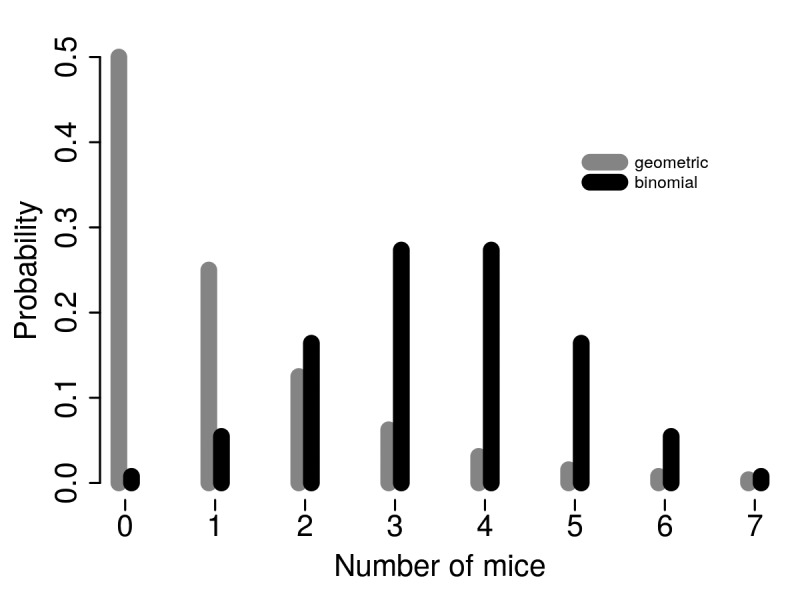
\includegraphics[width=\textwidth]{images/mouse_experiment_outcome.jpg}
      \caption{The experimental outcomes for the mice-population experiments as was taken from~\cite{ref:hackenberger:2019} .}
      \label{fig:probability:bayesian_statistics:mouse_experiment_outcome}
\end{figure}

If Bayesian statistics is used then the experimental design that was chosen does not matter. In Bayesian statistics it is common to use a Beta distribution as a prior distribution. If the prior distribution is sampled from $Beta(3,3)$ then using Bayesian analysis, the posterior distribution, according to the outcomes of this experiment, would yield $Beta(9,4)$. The process by which this is done is shown later in this section. The $Beta$ distribution was presented in Section \ref{sec:probability:probability_distributions:beta}.~\citeauthor{ref:hackenberger:2019}~\cite{ref:hackenberger:2019} mentions that the $Beta$ distribution can be seen as a probability distribution of the occurrence of specific parameters. From the information that is now known about the $Beta$ distribution, it is possible to calculate the probability that the sex ratio in this mice population is not 1:1 with the $Beta$ distribution as a prior, yielding a $P$-value of $0.92$. This means that there is a probability of $92\%$ that the mice population is not 1:1, regardless of experiment design. This is illustrated in Figure \ref{fig:probability:bayesian_statistics:mouse_distributions} below.

\begin{figure}[htbp]
      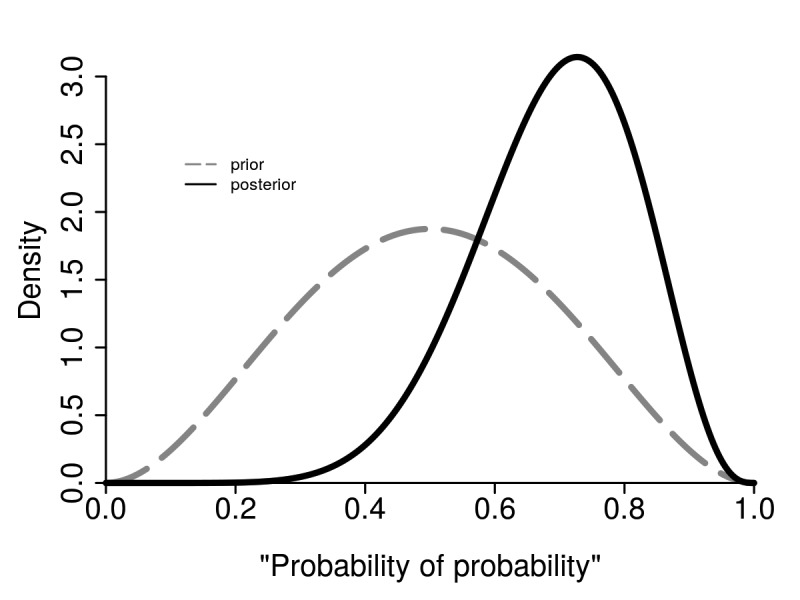
\includegraphics[width=\textwidth]{images/mouse_experiment_distributions.jpg}
      \caption{An illustration of the prior and posterior probability distributions for the outcomes of the mice-population experiment, using a $Beta$ prior, as was taken from~\cite{ref:hackenberger:2019}.}
      \label{fig:probability:bayesian_statistics:mouse_distributions}
\end{figure}

One can see from Figure \ref{fig:probability:bayesian_statistics:mouse_distributions} how the posterior distribution differs from the prior distribution. This is the nature of Bayesian analysis and is presented in more detail next.

\subsection{Bayesian Analysis}
\label{sec:probability:bayesian_statistics:bayesian_analysis}

Bayesian analysis is the process by which prior beliefs are updated as a result of observing new data/evidence. Similar to the approaches followed above to explain Bayesian statistics, a proposal is made to explain Bayesian analysis by means of an example taken from~\cite{ref:wackerly:2014}. Let $Y_{1}, Y_{2}, \dots, Y_{N}$ denote the random variable that is observed over a sample size of $N$. Then the likelihood of the sample is given as $\mathcal{L}(y_{1}, y_{2}, \dots, y_{n} \vert \theta)$. In the discrete case this function is defined to be the joint probability $P(Y_{1} = y_{1}, Y_{2} = y_{2}, \dots, Y_{N} = y_{n})$ and the continuous case yields the joint density of $Y_{1}, Y_{2}, \dots, Y_{N}$, evaluated at $y_{1}, y_{2}, \dots, y_{n}$. The Bayesian view models the parameter $\theta$ as a random variable with a probability distribution. This probability distribution is referred to as the prior distribution of $\theta$. The symbol $\theta$ is included in the notation of $\mathcal{L}$ as an argument to illustrate that this function is dependent explicitly on the value of $\theta$. Importantly, this prior distribution is specified before any data is collected and represents the theoretical prior knowledge about $\theta$. Assume that the parameter $\theta$ has a continuous distribution with density $g(\theta)$ that has no unknown parameters. Considering the likelihood of the data and the prior on $\theta$, then the joint likelihood of $Y_{1}, Y_{2}, \dots, Y_{N}, \theta$ is given in Equation~\eqref{eq:probability:bayesian_statistic:bayesian_analysis:joint_likelihood} below.

\begin{equation}
      \label{eq:probability:bayesian_statistic:bayesian_analysis:joint_likelihood}
      f(y_{1}, y_{2}, \dots, y_{n}, \theta) = \mathcal{L}(y_{1}, y_{2}, \dots, y_{n} \vert \theta)g(\theta)
\end{equation}

The marginal density or mass function of $Y_{1}, Y_{2}, \dots, Y_{N}$ is given in Equation~\eqref{eq:probability:bayesian_statistic:bayesian_analysis:marginal_density} below.

\begin{equation}
      \label{eq:probability:bayesian_statistic:bayesian_analysis:marginal_density}
      m(y_{1}, y_{2}, \dots, y_{n}) = \int_{-\infty}^{\infty} \mathcal{L}(y_{1}, y_{2}, \dots, y_{n} \vert \theta)g(\theta)d\theta
\end{equation}

Finally, the posterior density of $\theta \vert y_{1}, y_{2}, \dots, y_{n}$ according to Bayes' Theorem is given in Equation~\eqref{eq:probability:bayesian_statistic:bayesian_analysis:posterior_density} below.

\begin{equation}
      \label{eq:probability:bayesian_statistic:bayesian_analysis:posterior_density}
      g^{*}(\theta \vert y_{1}, y_{2}, \dots, y_{n}) = \frac{\mathcal{L}(y_{1}, y_{2}, \dots, y_{n} \vert \theta)g(\theta)}{\int_{-\infty}^{\infty} \mathcal{L}(y_{1}, y_{2}, \dots, y_{n} \vert \theta)g(\theta)d\theta}
\end{equation}

\citeauthor{ref:wackerly:2014}\cite{ref:wackerly:2014} mentions that the posterior density summarises all the pertinent information about the parameter $\theta$ by making use of the information contained in the prior for $\theta$ as well as the information in the observed data/evidence. Consider now how Bayesian analysis can used to update the priors on $\theta$ based on newly observed data. As with the example above, the below is taken from~\cite{ref:wackerly:2014}.

Let $Y_{1}, Y_{2}, \dots, Y_{N}$ denote a random sample from a $Bernoulli$ distribution where $P(Y_{i} = 1) = \theta$ and $P(Y_{i} = 0) = 1 - \theta$ and the prior distribution for $\theta$ is $Beta(\alpha, \beta)$. The formulation of the posterior distribution for $p$ is then shown as follows. Since the $Bernoulli$ probability function can be written as

\begin{equation*}
      P(y_{i} \vert \theta) = \theta^{y_{i}}(1 - \theta)^{1-y_{i}}
\end{equation*}

where $y_{i} = \{0,1\}$ and $0 < \theta < 1$. The likelihood $\mathcal{L}(y_{1}, y_{2}, \dots, y_{n} \vert \theta)$ is

\begin{equation*}
      \begin{split}
            \mathcal{L}(y_{1}, y_{2}, \dots, y_{n} \vert \theta)
            &= P(y_{1}, y_{2}, \dots, y_{n} \vert \theta)\\
            &= \theta^{y_{1}}(1-\theta)^{1 - y_{1}} \times \theta^{y_{2}}(1-\theta)^{1 - y_{2}} \times \dots \times \theta^{y_{n}}(1-\theta)^{1 - y_{n}}\\
            &= \theta^{\sum y_{i}}(1-\theta)^{n-\sum y_{i}}
      \end{split}
\end{equation*}

Then

\begin{equation*}
      \begin{split}
            f(y_{1}, y_{2}, \dots, y_{n}, \theta)
            &= \mathcal{L}(y_{1}, y_{2}, \dots, y_{n} \vert \theta)g(\theta)\\
            &= \theta^{\sum y_{i}}(1-\theta)^{n-\sum y_{i}} \times \frac{\Gamma(\alpha + \beta)}{\Gamma(\alpha)\Gamma(\beta)}\theta^{\alpha - 1}(1 - \theta)^{\beta  - 1}\\
            &= \frac{\Gamma(\alpha + \beta)}{\Gamma(\alpha)\Gamma(\beta)}\theta^{\sum y_{i} + \alpha - 1}(1-\theta)^{n - \sum y_{i} + \beta - 1}
      \end{split}
\end{equation*}

The marginal density of $Y_{1}, Y_{2}, \dots Y_{N}$ is then given as

\begin{equation*}
      \begin{split}
            m(y_{1}, y_{2}, \dots, y_{n})
            &= \int_{0}^{1}\frac{\Gamma(\alpha + \beta)}{\Gamma(\alpha)\Gamma(\beta)}\theta^{\sum y_{i} + \alpha - 1}(1-\theta)^{n - \sum y_{i} + \beta - 1}d\theta\\
            &= \frac{\Gamma(\alpha + \beta)}{\Gamma(\alpha)\Gamma(\beta)}\frac{\Gamma(\sum y_{i} + \alpha)\Gamma(n - \sum y_{i} + \beta)}{\Gamma(n + \alpha + \beta)}
      \end{split}
\end{equation*}

Finally, the posterior density of $\theta$ is given as

\begin{equation*}
      \begin{split}
            g^{*}(\theta \vert y_{1}, y_{2}, \dots, y_{n})
            &= \frac{\frac{\Gamma(\alpha + \beta)}{\Gamma(\alpha)\Gamma(\beta)}\theta^{\sum y_{i} + \alpha - 1}(1-\theta)^{n - \sum y_{i} + \beta - 1}}{\frac{\Gamma(\alpha + \beta)}{\Gamma(\alpha)\Gamma(\beta)}\frac{\Gamma(\sum y_{i} + \alpha)\Gamma(n - \sum y_{i} + \beta)}{\Gamma(n + \alpha + \beta)}}\\
            &= \frac{\Gamma(n + \alpha + \beta)}{\Gamma(\sum y_{i} + \alpha)\Gamma(n - \sum y_{i} + \beta)}\theta^{\sum y_{i} + \alpha - 1}(1-\theta)^{n - \sum y_{i} + \beta - 1}
      \end{split}
\end{equation*}

From the above, one can see that the posterior density has the same functional shape $\mathcal{A}(v)$ as the prior, yielding the update on prior parameters as $\alpha^{*} = \sum y_{i} + \alpha$ and $\beta^{*} = n - \sum y_{i} + \beta$.

\section{Summary}
\label{sec:probability:summary}

This chapter provided the reader with all the necessary background on probability theory and statistics that is required to formulate the \ac{BHH}. Detailed mathematical descriptions have been provided on probability distributions and proofs of conjugate priors are provided with detailed mathematical descriptions. Bayesian statistics have been presented in detailed and finally, it has been shown how Bayesian analysis works. The formulation of the \ac{BHH} is provided in the next chapter.